\section{System Modelling}\label{sec:modelling}
The kitticopter is a single mass moving vertically under three forces: rotor thrust, aerodynamic
drag and gravity. This section builds the model that the rest of the report rests on. It starts
from the forces, reaches a differential equation, and converts that equation into the transfer
functions used to design the controller. The model is left in terms of three constants that
cannot be derived from the brief and have to be measured on the system itself: the plant gain
$A$, the time constant $T$ and the sensor constant $k$. Section~\ref{sec:system_id} measures
them.

\subsection{Forces on the kitticopter}
Figure~\ref{fig:fbd} shows the three forces. Upwards is taken as positive, so the position
$y(t)$, the velocity $\dot{y}(t)$ and the thrust $f_t(t)$ are all positive upwards, while weight
acts downwards and drag acts against whichever way the kitticopter is moving.

\begin{figure}[htbp]
    \centering
    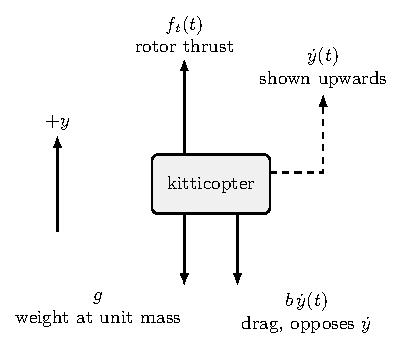
\includegraphics[width=0.34\textwidth]{figures/fbd.pdf}
    \caption{Free-body diagram of the kitticopter. Rotor thrust $f_t$ acts upwards, weight $g$
    acts downwards, and drag $b\dot{y}$ opposes the velocity. Upwards is positive.}
    \label{fig:fbd}
\end{figure}

Three modelling decisions come from the brief and each is used later.

\begin{enumerate}
    \item \textbf{Everything is normalised to the mass.} Newton's second law reads
    $m\ddot{y} = f_t - b_{\text{phys}}\dot{y} - mg$; dividing by $m$ and setting $m = 1$ folds
    the mass into every coefficient, so the thrust term is already an acceleration, $b$ has
    units of $\mathrm{s^{-1}}$ and $a$ has units of $\mathrm{m\,s^{-2}}$ per volt. Without
    stating this the units in the transfer function do not balance.
    \item \textbf{Drag is proportional to velocity and opposes it.} This keeps the model linear
    and first order in velocity, which is what makes it identifiable from a step test.
    \item \textbf{Gravity is a constant disturbance at the input.} It depends on neither position,
    velocity nor thrust, so it adds a fixed term to the acceleration rather than to the dynamics.
    That is why a fixed bias cancels it, and why the controller output is offset by the hover
    voltage rather than starting from zero.
\end{enumerate}

\subsection{Equation of motion}
Summing the forces of Figure~\ref{fig:fbd} at unit mass gives the acceleration of the
kitticopter,
\begin{equation}\label{eqn:eom}
    \ddot{y}(t) = a\,f_t(t) - b\,\dot{y}(t) - g ,
\end{equation}
with $g = 9.81\ \mathrm{m\,s^{-2}}$. The minus sign on the drag term is the statement that drag
opposes motion, and the minus sign on $g$ is the sign convention of Figure~\ref{fig:fbd}. Both
$a$ and $b$ are unknown at this stage.

\subsection{The controlled system and its interfaces}
The kitticopter is simulated while the controller is a physical circuit, so the loop crosses
between the two twice. The command is a voltage setting the angle of attack of the rotor blades,
entering through an ADC that accepts $0$ to $5\ \mathrm{V}$ with the midpoint calibrated to the
thrust that cancels gravity. Position leaves through a DAC and the sensor constant $k$, and since
the summing junction compares voltages, the same $k$ converts the setpoint from metres to volts.

\begin{figure}[htbp]
    \centering
    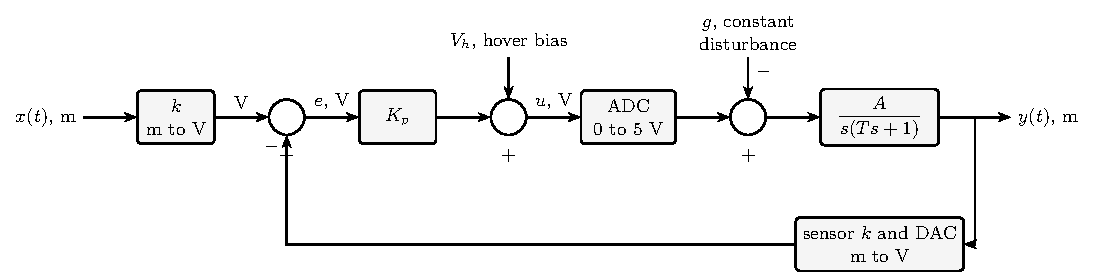
\includegraphics[width=0.85\textwidth]{figures/blockdiagram.pdf}
    \caption{Block diagram of the closed loop. The setpoint $x(t)$ in metres is converted to
    volts by $k$, compared with the fed-back sensor voltage, and the error is amplified by
    $K_p$. The hover bias $V_h$ is added at a separate summing junction so that the command
    $u(t)$ sits inside the $0$ to $5\ \mathrm{V}$ window the plant accepts. Gravity enters as a
    constant disturbance at the plant input, the same node the command arrives at.}
    \label{fig:blockdiagram}
\end{figure}

Two features of Figure~\ref{fig:blockdiagram} are used throughout. Gravity is summed at the plant
\emph{input}, not the output, and the level shift is its own summing junction rather than being
folded into $K_p$. Keeping it separate is what lets the gain be chosen on dynamic grounds alone
while the bias is trimmed independently.

\subsection{Transfer functions}
\subsubsection{Open loop}
Let $v = \dot{y}$ and treat gravity as the disturbance it is. Equation~\eqref{eqn:eom} then
reduces to $\dot{v} = a f_t - b v$, and with zero initial conditions,
\begin{equation}\label{eqn:openloop_vel}
    \frac{V(s)}{F_t(s)} = \frac{a}{s + b} = \frac{A}{Ts + 1},
    \qquad A = \frac{a}{b}, \qquad T = \frac{1}{b} .
\end{equation}

Working at velocity level is deliberate. At position level the pole at the origin means a step
drives the output away without settling, so there is no steady state from which to read a gain.
Differentiating the position gives Equation~\eqref{eqn:openloop_vel}, which has a finite final
value, so one step test fixes both unknowns: the gain from the settled velocity, the time constant
from how fast it is reached.

Position follows by integrating the velocity, which returns the pole at the origin:
\begin{equation}\label{eqn:openloop_pos}
    G(s) = \frac{Y(s)}{F_t(s)} = \frac{A}{s(Ts + 1)} .
\end{equation}

\subsubsection{Closed loop}
With gain $K_p$ and the sensor constant $k$ on both the feedback path and the reference
conversion, the loop gain is
\begin{equation}\label{eqn:loopgain}
    L(s) = \frac{K_p k A}{s(Ts + 1)} ,
\end{equation}
and the closed loop from setpoint to position, both in metres, is
\begin{equation}\label{eqn:closedloop}
    G_{cl}(s) = \frac{Y(s)}{X(s)} = \frac{K_p k A}{Ts^2 + s + K_p k A} .
\end{equation}

Dividing through by $T$ puts Equation~\eqref{eqn:closedloop} in the standard second-order form
$\omega_n^2 / (s^2 + 2\zeta\omega_n s + \omega_n^2)$, from which
\begin{equation}\label{eqn:wn_zeta}
    \omega_n = \sqrt{\frac{K_p k A}{T}},
    \qquad
    \zeta = \frac{1}{2\sqrt{T K_p k A}} .
\end{equation}

Equation~\eqref{eqn:wn_zeta} is the whole design problem in one line. Once the plant is
measured, $K_p$ is the only free parameter, and raising it raises $\omega_n$ while lowering
$\zeta$. Speed and overshoot therefore trade directly against one another, and
Section~\ref{sec:design} does nothing more than find the range of $K_p$ where both stay inside
the specification.

\subsection{Error, disturbance and type number}
The open loop of Equation~\eqref{eqn:openloop_pos} carries one free integrator, so the system is
type 1, and the final value theorem fixes two things before any gain is chosen. A step setpoint is
tracked with zero steady-state error, so the tracking half of the $8$ percent specification is met
by the structure rather than by tuning. A constant input disturbance, which is what gravity is,
leaves a finite offset
\begin{equation}\label{eqn:fvt_dist}
    y_{ss} = \frac{\Delta V}{K_p k} ,
\end{equation}
per volt of uncancelled input. No $K_p$ removes it, which is why the level shift exists and why
the whole $8$ percent budget is spent on the disturbance. Both closed-loop transfer functions are
derived in Appendix~\ref{sec:appendix}.

The structure is fixed; three constants are not. The gain $A$, the time constant $T = 1/b$ set by
drag, and the sensor constant $k$ are unique to this kitticopter.
Section~\ref{sec:system_id} measures them and Section~\ref{sec:design} uses them in
Equation~\eqref{eqn:wn_zeta} to choose $K_p$.
